\chapter{\MakeUppercase{System Design}}

\section{System Architecture}

This repository implements a modular experiment pipeline built to answer one practical question: how much fairness can we improve in credit scoring before predictive performance starts to drop too much?

Instead of treating model training as a single black box, the workflow is split into clear modules. This makes the project easier to understand, test, extend, and explain.

\begin{figure}[h!]
    \centering
    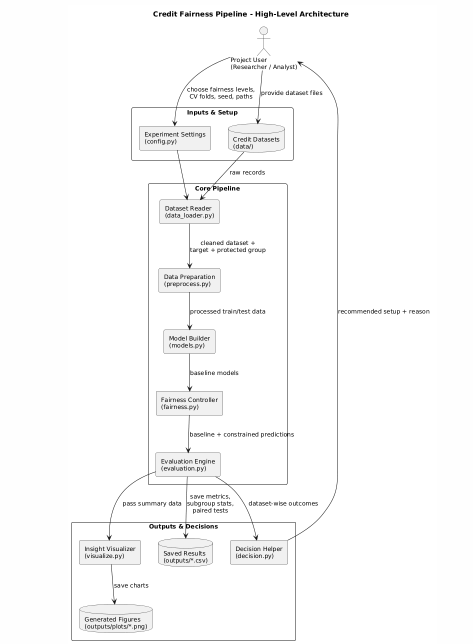
\includegraphics[width=0.85\textwidth]{images/system_architecture.png}
    \caption{High-Level Architecture Flow}
    \label{fig:system_architecture}
\end{figure}

\paragraph{Architecture Components Description}

\textbf{Data Ingestion and Preprocessing Module} \\
The system reads credit datasets from the data folder using dataset-specific loaders in \texttt{data\_loader.py}. At present, the implemented loaders support German Credit, Australian Credit, and GMSC.

It prepares the target label and protected group column, handles missing values, encodes categorical features, scales numeric features, and keeps preprocessing consistent across experiments. This consistency is important, because fair comparison between models is only possible when the input pipeline is controlled.

\vspace{0.5em}

\textbf{Model Training Module} \\
The project trains a range of models from simple to more expressive ones (\texttt{models.py}): Logistic Regression, Decision Tree, Random Forest, Gradient Boosting, Explainable Boosting Machine (EBM), and XGBoost.

All models are trained under the same experimental setup so that differences in results reflect model behavior, not setup noise.

\vspace{0.5em}

\textbf{Fairness Constraint Application Module} \\
Fairness intervention is handled through Fairlearn’s Exponentiated Gradient method (\texttt{fairness.py}). The system tests multiple fairness severity levels (from baseline to stronger constraint) defined in configuration.

The active constraint in this implementation is Demographic Parity. This stage allows explicit study of the fairness-performance trade-off.

\vspace{0.5em}

\textbf{Evaluation and Statistical Analysis Module} \\
After training, the system computes predictive metrics: Accuracy, ROC-AUC, and F1 Score. It also computes fairness metrics: Demographic Parity Difference, Equalized Odds Difference, and Disparate Impact Ratio.

To keep results statistically meaningful, the pipeline includes stratified cross-validation, confidence interval reporting, and paired t-tests between baseline and fairness-constrained settings.

Outputs are saved as structured CSV artifacts for reproducibility and later reporting.

\vspace{0.5em}

\textbf{Visualization and Trade-off Analysis Module} \\
The visualization module (\texttt{visualize.py}) turns raw results into readable evidence: fairness-accuracy trade-off curves, Pareto frontiers, combined scatter comparisons, and baseline-vs-mitigated charts.

These plots make it easier to communicate findings to both technical and non-technical stakeholders.

\vspace{0.5em}

\textbf{Decision Recommendation Module} \\
The recommendation logic (\texttt{decision.py}) helps select a practical configuration for each dataset. It balances fairness gains against acceptable accuracy loss and generates a plain-language summary of why a choice is recommended.

This bridges the gap between “what the metrics say” and “what a decision-maker should do.”

% ================= DESIGN =================
\section{Detailed Design}

\begin{figure}[h!]
    \centering
    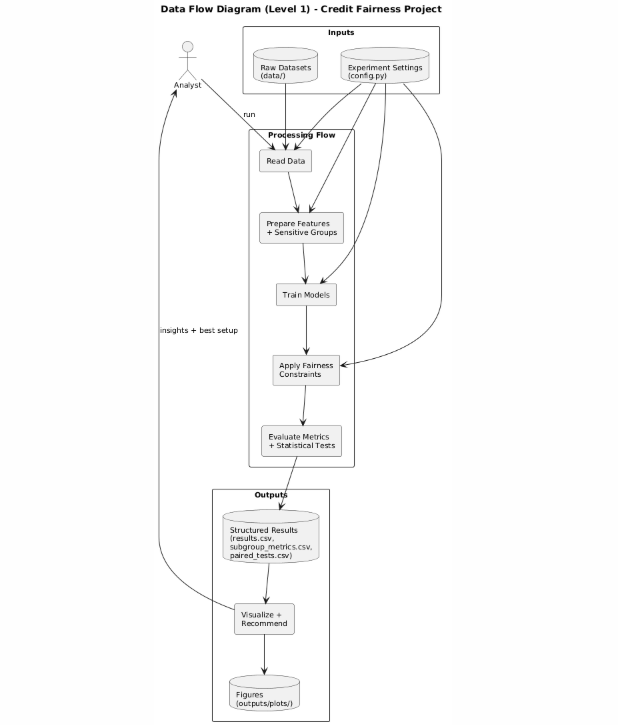
\includegraphics[width=0.9\textwidth]{images/dfd_level1.png}
    \caption{Data Flow Diagram (DFD Level 1)}
    \label{fig:dfd}
\end{figure}

\begin{figure}[h!]
    \centering
    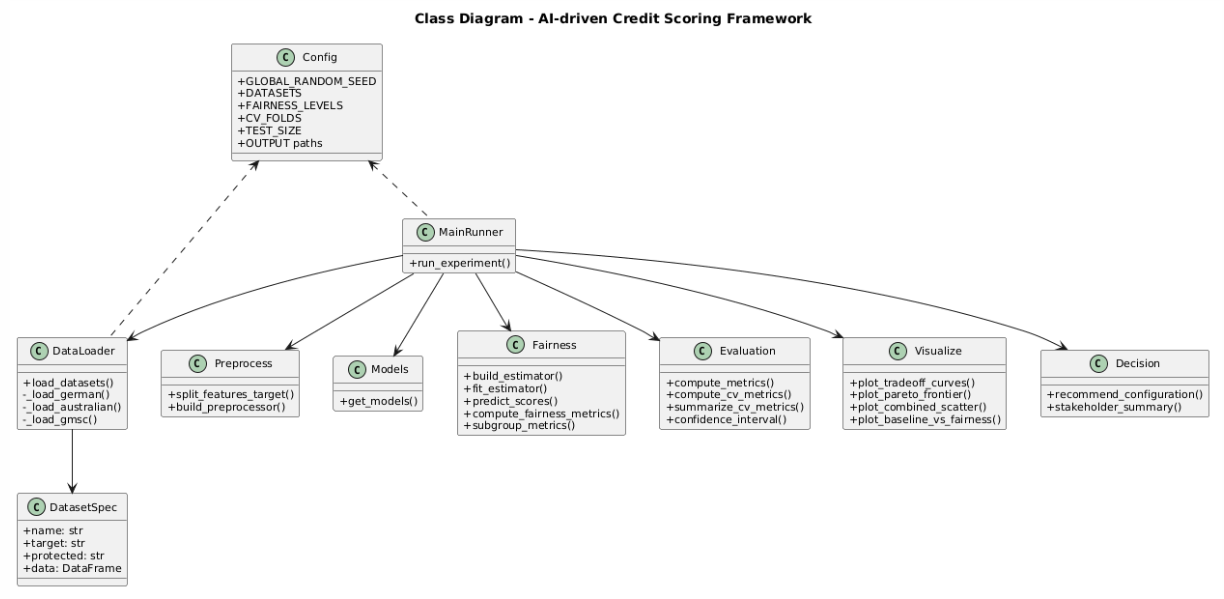
\includegraphics[width=0.9\textwidth]{images/class_diagram.png}
    \caption{Class Diagram}
    \label{fig:class_diagram}
\end{figure}

\paragraph{}

The detailed design of the system focuses on modularity and separation of concerns. Each major functionality is implemented as an independent module, allowing easier debugging, testing, and future extension.

The Data Flow Diagram (DFD Level 1) illustrates how data moves through the system—from dataset loading and preprocessing, through model training and fairness application, to evaluation and visualization.

The Class Diagram represents the structural design of the system, showing how different components such as data loaders, models, fairness handlers, and evaluation modules interact with each other. Each module encapsulates a specific responsibility, ensuring maintainability and scalability.

Together, these design representations provide both a process-level and structural-level understanding of the system.